\chapter{Data}
Data is collected for cryostat temperatures of $T\in\{ 2,4\}\ \si{\kelvin}$.
The \SI{2}{\kelvin} measurement features two series with $I_\text{sample}\in\{ 20,100\}\ \si{\micro\ampere}$, whereas the \SI{4}{\kelvin} measurement only features a series for $I_\text{sample}=\SI{20}{\micro\ampere}$.
The procedure for recordingone set of data is
\begin{enumerate}
	\item Adjust sample current and temperature.
	\item Record hall voltage while sweeping magnetic field up.
	\item Record longitudinal voltage while sweeping magnetic field down.
\end{enumerate}
A \texttt{PeakTech 12xx} digital oscilloscope is used to acquire voltage curves, which has to be replaced as soon as humanly possible.

\section{Methods} %TODO: Employed methods for data evaluation
\begin{figure}
	\centering
	\begin{subfigure}{.48\textwidth}
		\centering
		\includegraphics[width=\linewidth]{./data/plots/2K-20uA-hw.pdf}
		\caption{\textbf{Uncut data} Part of data is not recoverable and thus not evaluable.}
	\end{subfigure}
	\hspace*{\fill}
	\begin{subfigure}{.48\textwidth}
		\centering
		\includegraphics[width=\linewidth]{./data/plots/2K-20uA-unfiltered.pdf}
		\caption{\textbf{Unfiltered, cut data}}
	\end{subfigure}
	\caption[Comparison of (un)processed example data]{\textbf{Comparison of (un)processed example data}}
	\label{fig:comparison}
\end{figure}
\autoref{fig:comparison} shows a side-by-side comparison of example data prior to and after cutting.
It is easy to see that part of the data is corrupted and cannot be evaluated as a result of a data corruption while saving the trace to a file.
Therefore, the corrupted part is cut off and a Savitzky–Golay filter is applied to the data filter out high frequency noise.
Filtered data can be seen in \autoref{sec:plots} and will be discussed henceforth.

Since, in this setup, the magnetic field is recorded with the oscilloscope as well, the magnetic field is calculated from the voltage recorded by the oscilloscope using linear mapping.
This is obtained by comparing the difference between the lowest and highest recorded voltages of the curve with the maximum megnetic field set in the controller.

\section{Plots}\label{sec:plots}
\begin{figure}
	\centering
	\begin{subfigure}{.48\textwidth}
		\centering
		\includegraphics[width=\linewidth]{./data/plots/4K-20uA-main.pdf}
		\caption{$T=\SI{4}{\kelvin}, I_\text{samp} = \SI{20}{\micro\ampere}$}
	\end{subfigure}
	\hspace*{\fill}
	\begin{subfigure}{.48\textwidth}
		\centering
		\includegraphics[width=\linewidth]{./data/plots/2K-20uA-main.pdf}
		\caption{$T=\SI{2}{\kelvin}, I_\text{samp} = \SI{20}{\micro\ampere}$}
	\end{subfigure}
	\hspace*{\fill}
	\begin{subfigure}{.48\textwidth}
		\centering
		\includegraphics[width=\linewidth]{./data/plots/2K-100uA-main.pdf}
		\caption{$T=\SI{2}{\kelvin}, I_\text{samp} = \SI{100}{\micro\ampere}$}
	\end{subfigure}
	\hspace*{\fill}
	\caption[Plots for various settings]{\textbf{Plots for various settings}}
	\label{fig:plots}
\end{figure}
\autoref{fig:plots} shows all of the recorded data for different temperatures and sample currents.
The hall voltages show the expected plateau-behavior while the longitudinal voltages oscillate as suggested by theory established in \autoref{chap:theory}.
Plateau numbers shown in the plots are obtained by utilizing the relation
\begin{equation*}
	i = \left. \frac{R_\text{K}}{R_\text{hall}} \right\rvert_{\text{plat}} = R_\text{K}\cdot\left. \frac{I_\text{samp}}{U_\text{H}}\right\rvert_{\text{plat}}
\end{equation*}

\section{Longitudinal Voltages}
\begin{figure}
	\centering
	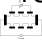
\includegraphics[width=.5\textwidth]{./img/setup_res.pdf}
	\caption[Setup for measuring longitudinal voltage]{\textbf{Setup for measuring longitudinal voltage} Probing points are selected by utilizing the provided rotary switches.}
	\label{fig:setup_long_don_jon}
\end{figure}

\begin{table}
	\caption[Longitudinal voltages]{\textbf{Longitudinal voltages}}
	\label{tabs:long}
\begin{minipage}[t]{.33\linewidth}
\caption{$T=\SI{4}{\kelvin}, I_\text{samp} = \SI{20}{\micro\ampere}$}  \label{tab:4k20}
\centering
		\begin{tabular}{SS}
		\toprule
		{B (\si{\tesla})} &       {U (\si{\mV})}    \\
		\midrule
		3.36    &       48 \\
		1.82    &       16 \\
		1.36    &       18 \\
		1.05    &       16 \\
		\bottomrule
		\end{tabular}%
\end{minipage}%
\hfill%
\begin{minipage}[t]{.33\linewidth}
	\caption{$T=\SI{2}{\kelvin}, I_\text{samp} = \SI{20}{\micro\ampere}$}\label{tab:2k20}
	\centering
		\begin{tabular}{SS}
		\toprule
		{B (\si{\tesla})} &       {U (\si{\mV})}    \\
		\midrule
		3.32    &       54 \\
		1.86    &       24 \\
		1.41    &       24 \\
		1.05    &       18 \\
		0.82    &       14 \\
		\bottomrule
		\end{tabular}%
\end{minipage}%
\hfill%
\begin{minipage}[t]{.33\linewidth}
	\caption{$T=\SI{2}{\kelvin}, I_\text{samp} = \SI{100}{\micro\ampere}$} \label{tab:2k100}
	\centering
		\begin{tabular}{SS}
		\toprule
		{B (\si{\tesla})} &       {U (\si{\mV})}    \\
		\midrule
		3.45    &       208 \\
		1.86    &       104 \\
		1.41    &       96 \\
		\bottomrule
		\end{tabular}
\end{minipage}
\end{table}
\autoref{tabs:long} shows the peak values of the longitudinal voltages and their corresponding magnetic flux densities collected using the setup shown in \autoref{fig:setup_long_don_jon}.
It is easy to see that more extreme values are visible for a sample current of $I_\text{samp}=\SI{20}{\micro\ampere}$ and a given range of the magnetic field $B\in[0,B_\text{cut}]$, where $B_\text{cut}$ is the magnetic field value at which the measurements begin to get corrupted.

\section{Hall Voltages} %TODO: Listing of hall voltages and their corresponding magnetic flux densities
\begin{figure}
	\centering
	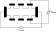
\includegraphics[width=.5\textwidth]{./img/setup_hall.pdf}
	\caption[Setup for measuring hall voltage]{\textbf{Setup for measuring hall voltage} Probing points are adjusted by utilizing the provided rotary encoders.}
	\label{fig:setup_hall_of_fame}
\end{figure}

\begin{table}
	\caption[Hall voltages]{\textbf{Hall voltages}}
	\label{tabs:hall}
\begin{minipage}[t]{\linewidth}
	\caption{$T=\SI{4}{\kelvin}, I_\text{samp} = \SI{20}{\micro\ampere}$}  \label{tab:4k20}
	\centering
	\begin{tabular}{SS|SS|S|S}
		\toprule
		{$B_\text{min}$ (\si{\tesla})}      &       {$B_\text{max}$ (\si{\tesla})}      &       {$\bar{U_\text{h}}$ (\si{\mV})}     &       {$\sigma(U_\text{h})$ (\si{\mV})}   &       {$i$}       &       {$R_\text{h}$ (\si{\ohm})}  \\
		\midrule
		1.32    &       1.44    &       90      &       3.0     &       6    &       4500.0 \\
		1.88    &       2.20    &       133     &       3.4     &       4    &       6653.1 \\
		3.40    &       4.80    &       264     &       3.5     &       2    &       13214.0 \\
		\bottomrule
	\end{tabular}
\end{minipage}%
\hfill%
\begin{minipage}[t]{\linewidth}
	\caption{$T=\SI{2}{\kelvin}, I_\text{samp} = \SI{20}{\micro\ampere}$}\label{tab:2k20}
	\centering
	\begin{tabular}{SS|SS|S|S}
		\toprule
		{$B_\text{min}$ (\si{\tesla})}      &       {$B_\text{max}$ (\si{\tesla})}      &       {$\bar{U_\text{h}}$ (\si{\mV})}     &       {$\sigma(U_\text{h})$ (\si{\mV})}   &       {$i$}       &       {$R_\text{h}$ (\si{\ohm})}  \\
		\midrule
		1.28    &       1.44    &       90      &       3.3     &       6    &       4513.5 \\
		1.84    &       2.28    &       134     &       3.3     &       4    &       6710.7 \\
		3.32    &       5.04    &       266     &       3.3     &       2    &       13281.7 \\
		\bottomrule
	\end{tabular}
\end{minipage}%
\hfill%
\begin{minipage}[t]{\linewidth}
	\caption{$T=\SI{2}{\kelvin}, I_\text{samp} = \SI{100}{\micro\ampere}$} \label{tab:2k100}
	\centering
	\begin{tabular}{SS|SS|S|S}
		\toprule
		{$B_\text{min}$ (\si{\tesla})}      &       {$B_\text{max}$ (\si{\tesla})}      &       {$\bar{U_\text{h}}$ (\si{\mV})}     &       {$\sigma(U_\text{h})$ (\si{\mV})}   &       {$i$}       &       {$R_\text{h}$ (\si{\ohm})}  \\
		\midrule
		1.96    &       2.16    &       664     &       6.0     &       4    &       6640.0 \\
		3.44    &       4.68    &       1315    &       6.4     &       2    &       13148.0 \\
		\bottomrule
	\end{tabular}
\end{minipage}
\hfill
\end{table}
\autoref{tabs:hall} shows the values for hall voltages at the plateaus and their corresponding magnetic flux densities collected using the setup shown in \autoref{fig:setup_hall_of_fame}.

\section{Charge Carrier Density}\label{sec:ccd} %TODO: Dito.
Assuming that all $N$ Landau levels are fully occupied, the relation
\begin{equation*}
	n_\text{cc} = \frac{2e}{h\cdot\Delta\left(\frac{1}{B}\right)}
\end{equation*}
may be used to calculate the charge carrier density $n_\text{cc}$ of the 2DEG, where $\Delta\left(\frac{1}{B}\right)$ is the measured period of the conductivity oscillations, observable in the oscillations of longitudinal voltages.
$\Delta\left(\frac{1}{B}\right)$ is obtained via linear regression of form $\frac{1}{B_\text{peaks}} = \Delta\left(\frac{1}{B}\right)\cdot i + b$, where subsequent values of $i$ have a distance of 2 from each other.

Applying these deliberations yields charge carrier density values of
\begin{align*}
	n\left(\SI{2}{\kelvin},\SI{20}{\micro\ampere}\right) &= \SI{4.439e11}{\per\centi\meter\squared} \\
	n\left(\SI{2}{\kelvin},\SI{100}{\micro\ampere}\right) &= \SI{4.203e11}{\per\centi\meter\squared} \\
	n\left(\SI{4}{\kelvin},\SI{20}{\micro\ampere}\right) &= \SI{4.224e11}{\per\centi\meter\squared},
\end{align*}
with a rather low standard deviation of \SI{1.31e10}{\per\meter\squared}. %yup, keeping this. whole point of computing the std

The mean value of found charge carrier densities is of no interest, since the quality of measurements carried out at different temperatures should differ vastly.
It is assumed that for lower temperatures less electrons will be excited into higher states of the triangular quantum well discussed in \autoref{sec:2deg-theory}.
Therefore, the quality of the used 2DEG will be higher at lower temperatures, increasing the significance of these results.

\section{Fine-Structure Constant}\label{sec:fine} %TODO: Why are you reading this?
To determine a value for the fine-structure constant, relations
\begin{equation*}
	R_\text{hall} = \left. \frac{U_\text{hall}}{I_\text{sample}}\right\rvert_\text{peaks}
\end{equation*}
and
\begin{equation*}
	\left. \frac{1}{R_\text{hall}}\right\rvert_\text{peaks} = \frac{2\alpha}{\mu_0 c}\cdot i
\end{equation*}
are used.

A linear regression of form
\begin{equation*}
	\left. \frac{1}{R_\text{hall}}\right\rvert_\text{peaks} = a\cdot i + b
\end{equation*}
is used to determine the slope $a=\frac{2\upalpha}{\mu_0 c}$.
Errors on measurements of $U_\text{hall}$ propagate into $R_\text{hall}$ like
\begin{equation*}
	\sigma_{R_\text{hall}} = \frac{\sigma_{U_\text{hall}}}{I_\text{sample}}
\end{equation*}
and finally into the y-errors of the linear regression like
\begin{equation*}
	\sigma_{R^{-1}_\text{hall}} = \frac{\sigma_{R_\text{hall}}}{R_\text{hall}^2}.
\end{equation*}

Carrying out linear regression and rearranging for $\alpha$ yields fine-structure constants of
\begin{align*}
	\alpha^{-1}_{\SI{2}{\kelvin},\SI{20}{\micro\ampere}} &= \num{145.18(733)} \\
	\alpha^{-1}_{\SI{2}{\kelvin},\SI{100}{\micro\ampere}} &= \num{142.43(578)} \\
	\alpha^{-1}_{\SI{4}{\kelvin},\SI{20}{\micro\ampere}} &= \num{144.91(704)}.
\end{align*}
Errors are propagated like
\begin{equation*}
	\sigma_{\alpha^{-1}} = \frac{\sigma_\alpha}{\alpha^2}\quad\text{, where}\quad\sigma_\alpha = \sigma_a\cdot\frac{\mu_0c}{2}
\end{equation*}
with the fit error $\sigma_a$ from the performed linear regression.
